  \documentclass[xcolor=table]{beamer}
\usepackage{beamerthemesplit}
\usepackage{wrapfig}
\usetheme{SPbGU}
\usepackage{pdfpages}
\usepackage{amsmath}
\usepackage{cmap} 
\usepackage[T2A]{fontenc} 
\usepackage[utf8]{inputenc}
\usepackage[english]{babel}
\usepackage{indentfirst}
\usepackage{amsmath}
\usepackage{tikz}
\usepackage{multirow}
\usepackage[noend]{algpseudocode}
\usepackage{algorithm}
\usepackage{algorithmicx}
\usepackage{fancyvrb}
\usetikzlibrary{shapes,arrows}
%usepackage{fancyvrb}
%\usepackage{minted}
%\usepackage{verbments}


\beamertemplatenavigationsymbolsempty

\title[Parsing techniques for graph analysis]{Parsing techniques for graph analysis}
\institute[SPbU]{
JetBrains Research, Programming Languages and Tools Lab  \\
Saint Petersburg University
}

\author[Kate Verbitskaia]{Semyon Grigorev, \textbf{Kate Verbitskaia}}

\date{October 22, 2017}

\definecolor{orange}{RGB}{179,36,31}

\begin{document}
{
\begin{frame}[fragile]
  \begin{tabular}{p{3.5cm} p{5.5cm} p{1cm}}
   \begin{center}
      
\includegraphics[height=1.5cm]{pictures/jetbrainsResearch.pdf}
    \end{center}
    &
    \begin{center}
      
\includegraphics[height=1.5cm]{pictures/SLELogo.png}
    \end{center}
    &
    \begin{center}
      
\includegraphics[height=1.5cm]{pictures/SPbGU_Logo.png}
    \end{center} 
  \end{tabular}
  \titlepage
\end{frame}
}

\begin{frame}[fragile]
  \transwipe[direction=90]
  \frametitle{Language-constrained path filtering}
  \begin{minipage}[m]{0.45\linewidth}
\raisebox{-0.5\totalheight}{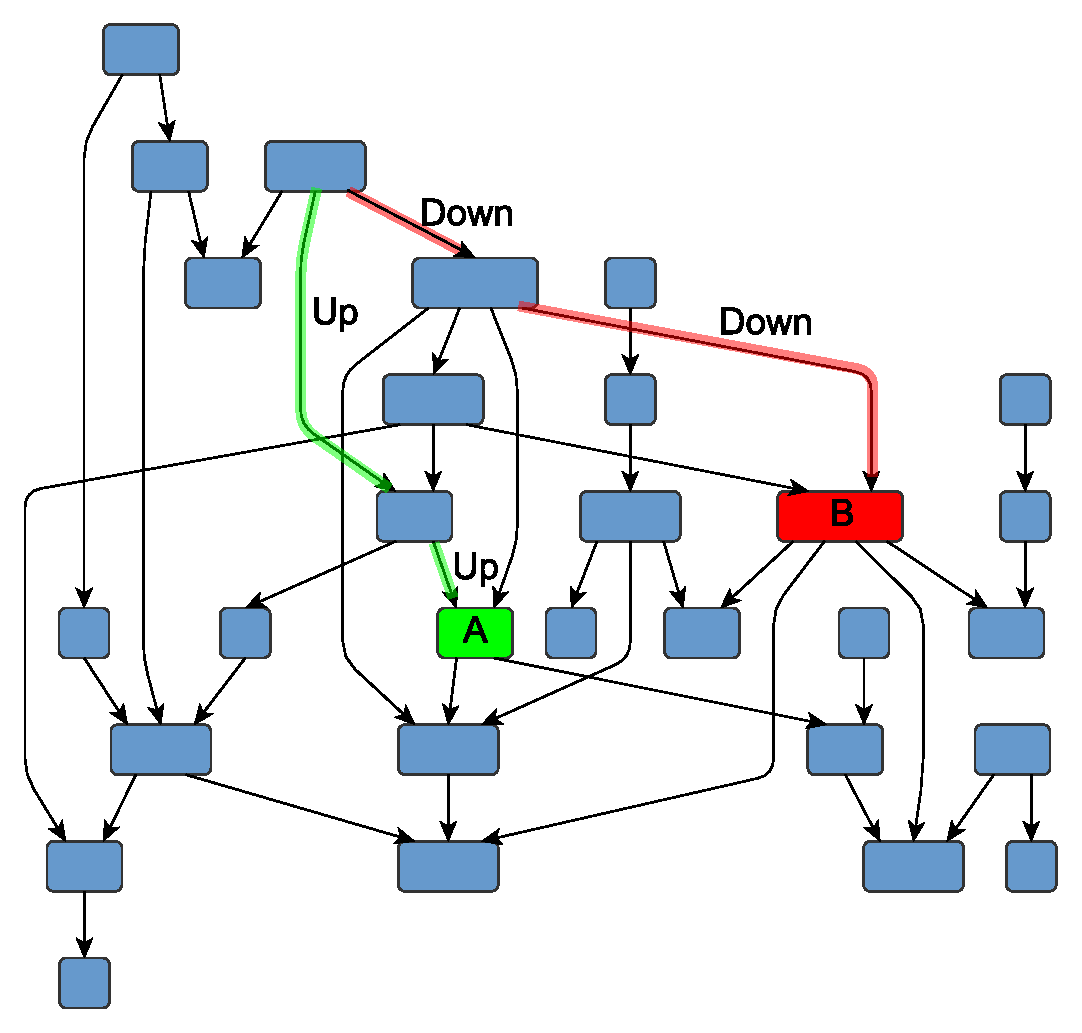
\includegraphics[width=\textwidth]{pictures/hierarchical.pdf}}
\end{minipage}\hfill
\begin{minipage}[m]{0.5\linewidth}
Navigation through a graph
\begin{itemize}
      \item Are nodes A and B on the same level of hierarchy?
      \item Is there a path of form $\textbf{Up}^n \, \textbf{Down}^n$?
      \item Find all paths of form $\textbf{Up}^n \, \textbf{Down}^n$ which start from the~node A
\end{itemize}

\end{minipage}

  \begin{itemize}
    \item (How) Can an automaton generate phrases in some specific (context-free) language?
    \item (How) Can a program produce some specific chain of the subprogram calls? 
  \end{itemize}
\end{frame}

\begin{frame}[fragile]
  \transwipe[direction=90]
  \frametitle{Language-constrained path filtering: more formal}
  \begin{itemize}
    \item $\mathbb{G} = (\Sigma, N, P)$ --- context-free grammar
    \item $G = (V,E,L)$ --- directed graph
      \begin{itemize} 
        \item $v \xrightarrow{l} u \in E$
        \item $L\subseteq \Sigma$
      \end{itemize}
    %\item $p = v_0 \xrightarrow{l_0} v_1 \xrightarrow{l_1} \cdots \xrightarrow{l_{n-2}} v_{n-1} \xrightarrow{l_{n-1}} v_n$ --- path in $G$
    \item $\omega(p) = \omega(v_0 \xrightarrow{l_0} v_1 \xrightarrow{l_1} \cdots \xrightarrow{l_{n-2}} v_{n-1} \xrightarrow{l_{n-1}} v_n) = l_0 l_1 \cdots l_{n-1}$
    \item $R = \{ p \mid $ exists $ N_i \in N $ such that $ \omega(p) \in L(\mathbb{G},N_i)\}$
  \end{itemize}
\end{frame}

\begin{frame}[fragile]
  \transwipe[direction=90]
  \frametitle{Applications}
  \begin{itemize}
    \item Graph database querying (\href{http://dl.acm.org/citation.cfm?id=298576}{Yannakakis.~1990}; \href{https://uhdspace.uhasselt.be/dspace/handle/1942/16709}{Hellings.~2014}; \href{https://link.springer.com/chapter/10.1007/978-3-319-46523-4_38}{Zhang.~2016})
    \item Сode analysis
    \begin{itemize}
      \item Static analysis via context-free and linear conjunctive language reachability
        \begin{itemize}
          \item alias analysis (\href{https://dl.acm.org/citation.cfm?id=3009848}{Zhang, Su. 2017})
          \item points-to analysis (\href{https://link.springer.com/chapter/10.1007/978-3-642-03013-0_6}{Xu, Rountev, Sridharan. 2009})
        \end{itemize}
      \item Dynamically generated strings analysis (\href{https://link.springer.com/chapter/10.1007/978-3-319-41579-6\_22}{Verbitskaia, Grigorev, Avdyukhin. 2015})
      \item Multiple input parsing (\href{https://2016.splashcon.org/event/parsing2016-multiple-input-gll-parsing}{Scott, Johnstone. 2016})
    \end{itemize}
    \item \dots
  \end{itemize}
\end{frame}

\begin{frame}
  \transwipe[direction=90]
  \frametitle{Existing approaches}
  \begin{itemize}
    \item Do not use the power of advanced parsing techniques
    \begin{itemize}
       \item Are mostly based on CYK \\ (Zhang, et al. ``Context-free path queries on RDF graphs.''; \\ Hellings. ``Conjunctive context-free path queries.'')
       \item Do not provide useful structural representation of result
     \end{itemize}
    \item Impose restrictions on input
    \begin{itemize}
       \item Do not process input graphs with cycles \\ (Sevon, Eronen. ``Subgraph queries by context-free grammars.'')
       \item Are restricted to certain grammar classes
     \end{itemize}
  \end{itemize}
\end{frame}

\begin{frame}
  \transwipe[direction=90]
  \frametitle{Open problems}
  \begin{itemize}
    \item Development of efficient algorithms
    \item Result representation for query debugging and further processing 
    \item Processing of various types of grammars (ECFG, conjunctive, etc)
  \end{itemize}
\end{frame}

%\begin{frame}
%  \transwipe[direction=90]
%  \frametitle{Bar-Hillel theorem}
%  \begin{itemize}
%    \item Context-free languages are closed under intersection with regular languages
%    \item Parsing algorithms are constructive proof of Bar-Hillel theorem for one simple case \dots
%    \item \dots so, classical parsing can be generalized for arbitrary regular language processing
%  \end{itemize}
%\end{frame}

\begin{frame}
  \transwipe[direction=90]
  \frametitle{Example}
\begin{figure}[ht]
    \centering
        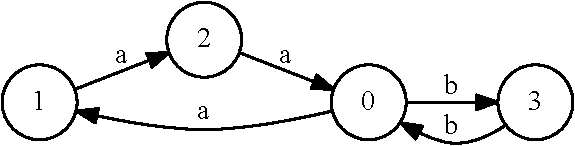
\includegraphics[width=0.45\textwidth]{pictures/input.pdf}\\
        Input graph
\end{figure}
\begin{figure}[ht]
\centering
   \[
\begin{array}{rrl} 
   S & \rightarrow & a \ S \ b \\
   S & \rightarrow & Middle \\
   Middle & \rightarrow & a \ b
\end{array}
\]
   Query: a grammar for the language $L=\{a^n b^n \mid n \geq 1\}$ with an additional marker for the middle of the path
   \label{grammarG}        
    \end{figure}
\end{frame}

\begin{frame}
  \transwipe[direction=90]
  \frametitle{Example}
\begin{figure}[ht]
    \centering
        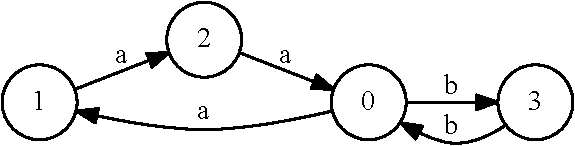
\includegraphics[width=0.45\textwidth]{pictures/input.pdf} \\
        Input graph
\end{figure}

\begin{overprint}

\onslide<1>
\begin{tabular}{  c  c  c  }
    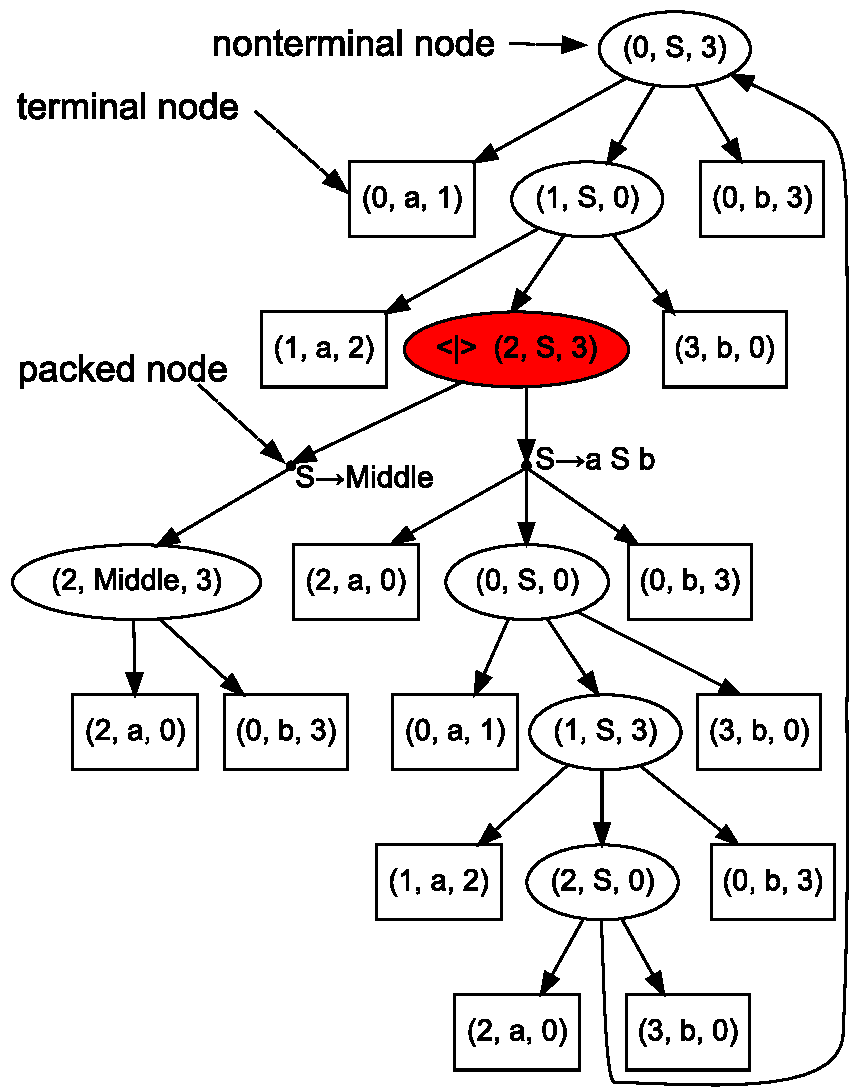
\includegraphics[height=4.5cm]{pictures/AnBn.pdf}
    &
    %
    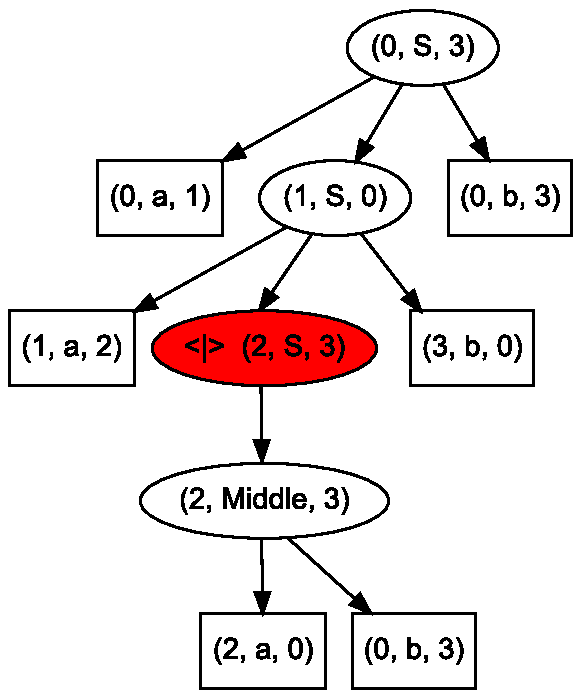
\includegraphics[height=4.5cm]{pictures/AnBn_2.pdf}
    %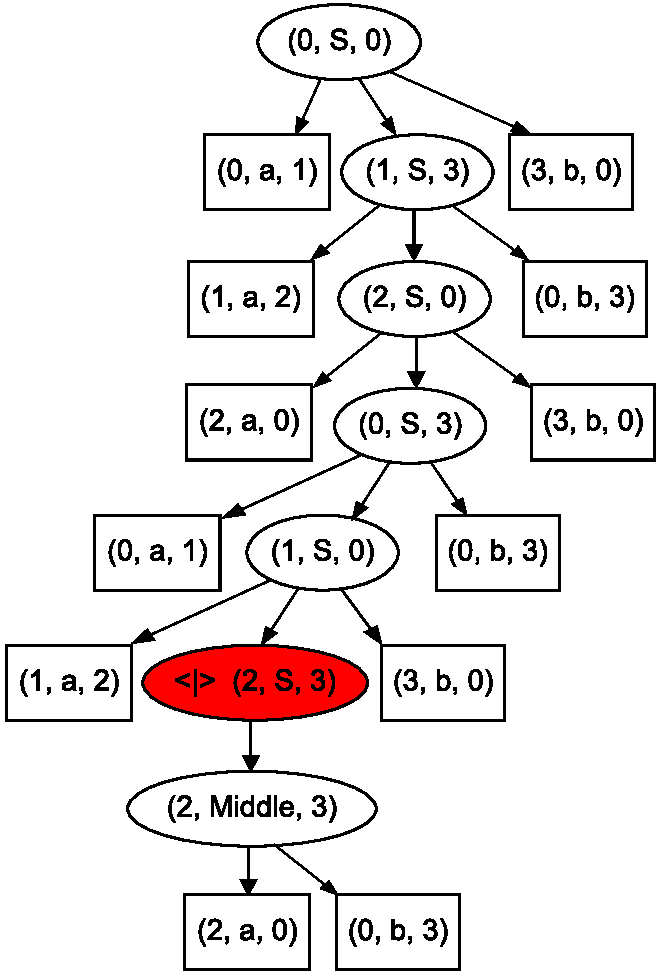
\includegraphics[height=4.5cm]{pictures/AnBn_1.pdf}
    %

    %\alt<1>{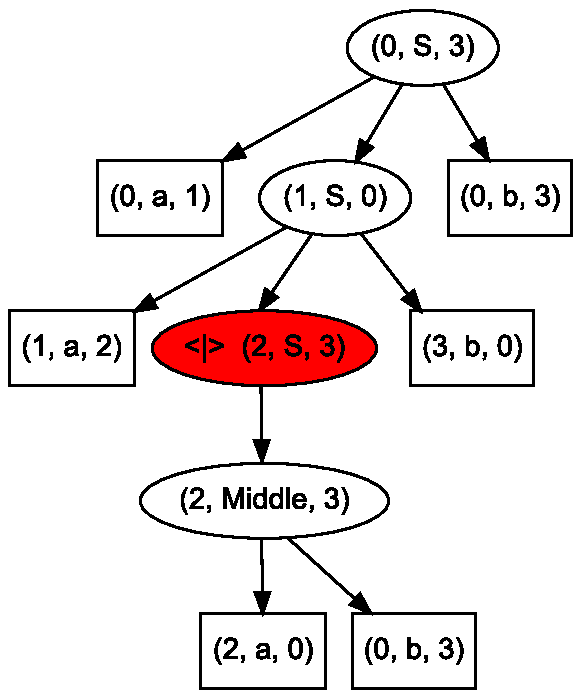
\includegraphics[height=4.5cm]{pictures/AnBn_2.pdf}}{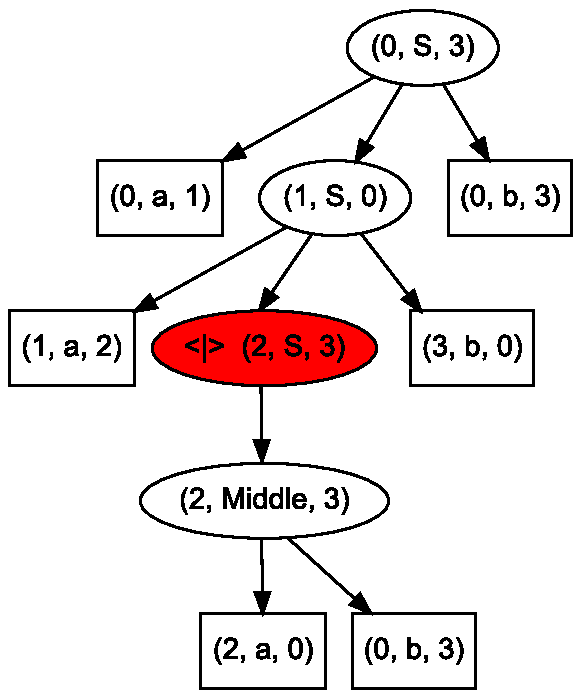
\includegraphics[height=4.5cm]{pictures/AnBn_2.pdf}}
    &
    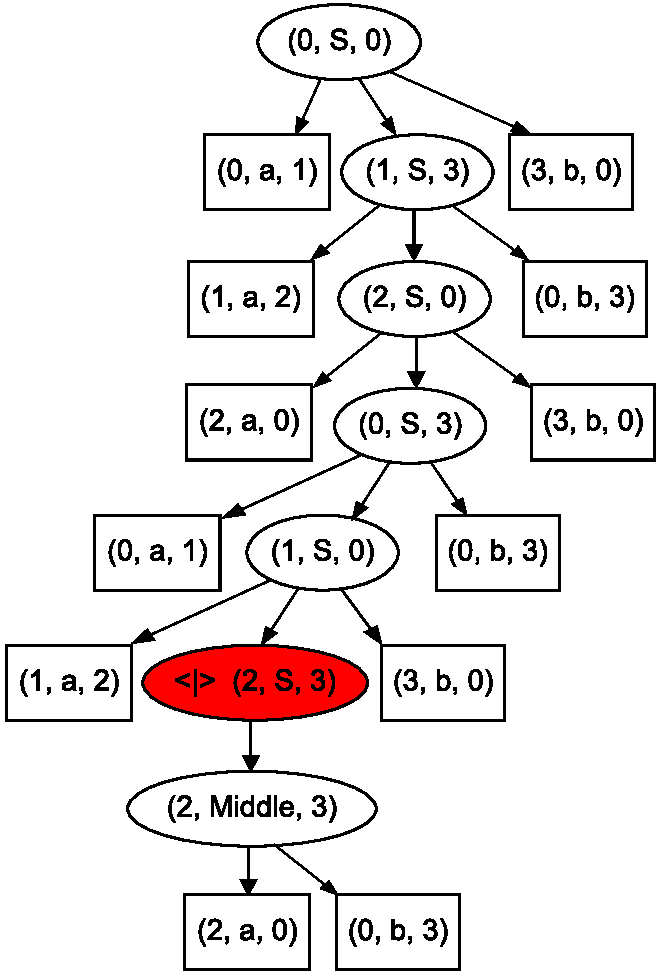
\includegraphics[height=4.5cm]{pictures/AnBn_1.pdf}

\\
\small{Query result: SPPF}
& \small{Tree for the path $0 \leadsto 3$}
& \small{Tree for the path $0 \leadsto 0$}
\end{tabular}
\onslide<2>
\begin{tabular}{  c  c  c  }
    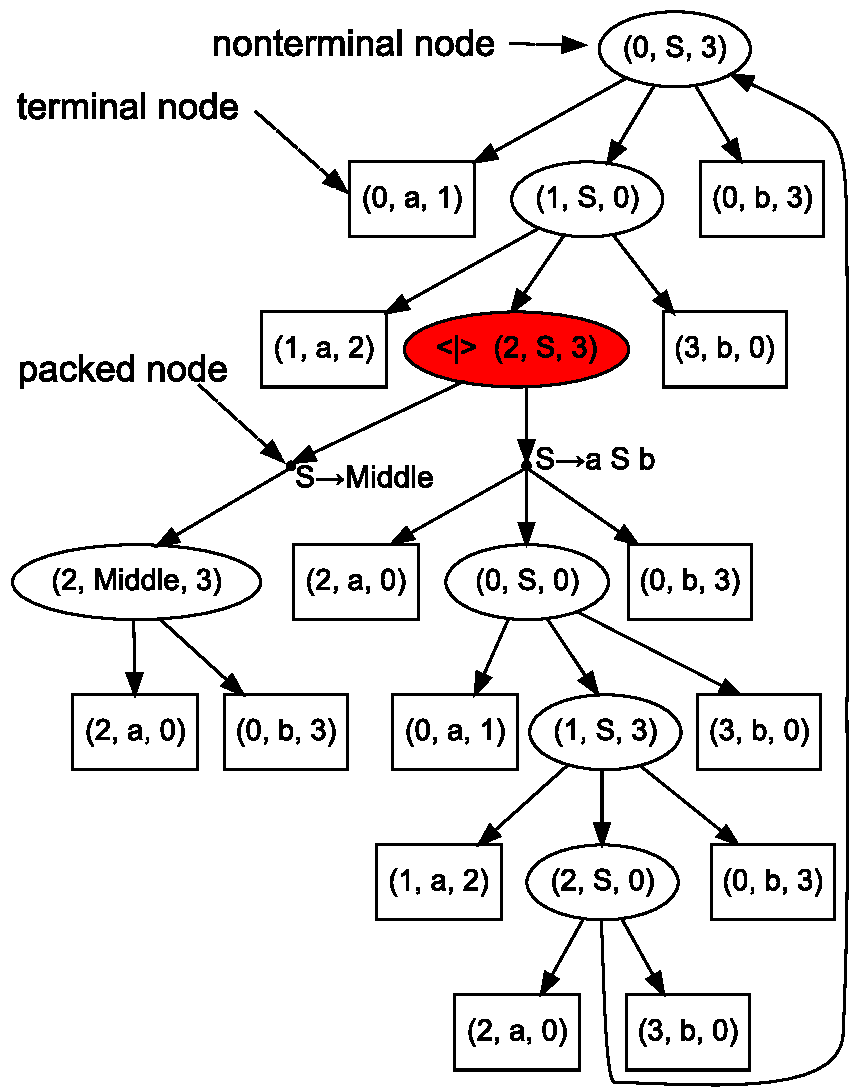
\includegraphics[height=4.5cm]{pictures/AnBn.pdf}
    &
    %
    %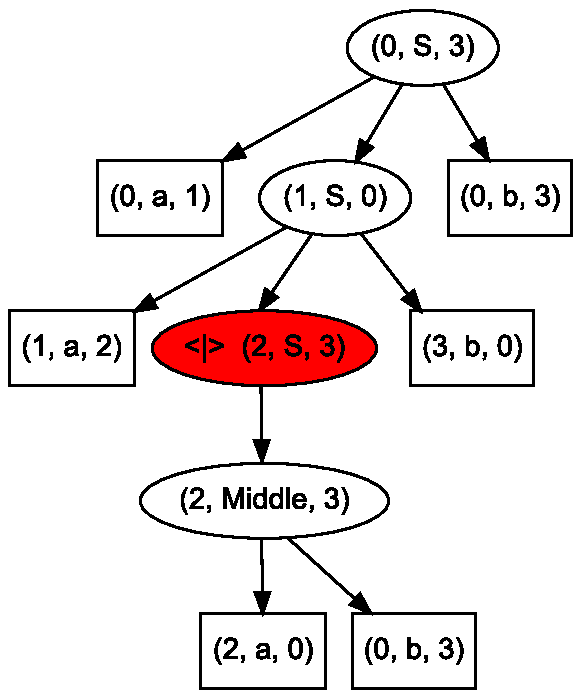
\includegraphics[height=4.5cm]{pictures/AnBn_2.pdf}
    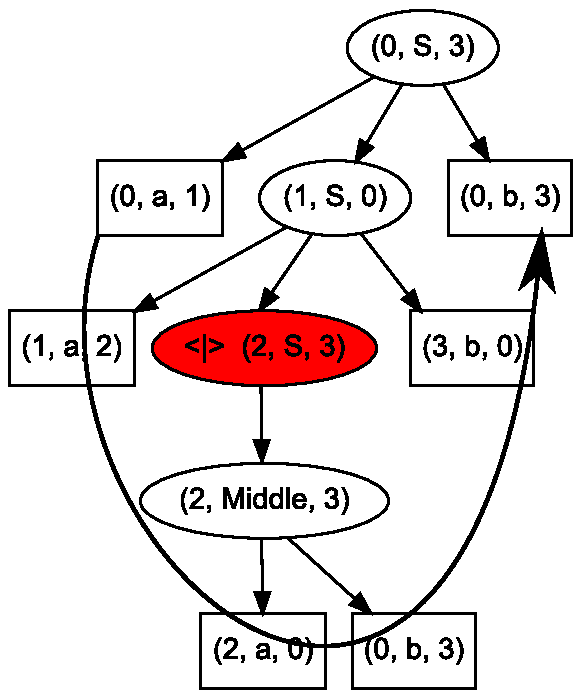
\includegraphics[height=4.5cm]{pictures/AnBn_2_m.pdf}
    %

    %\alt<1>{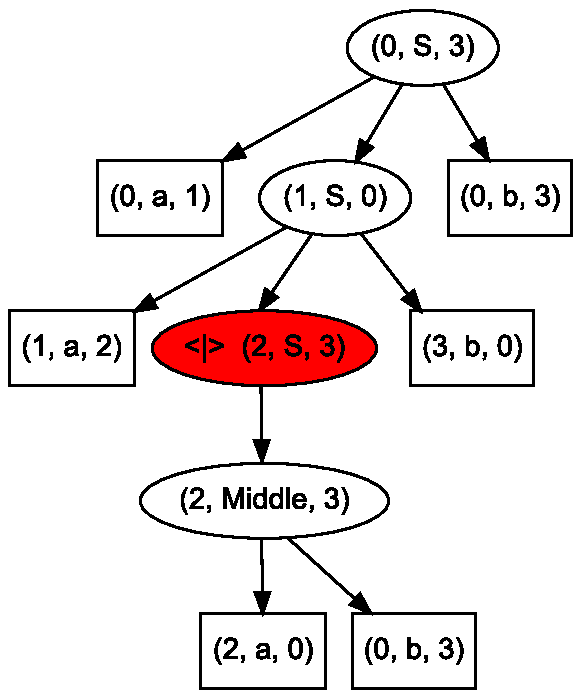
\includegraphics[height=4.5cm]{pictures/AnBn_2.pdf}}{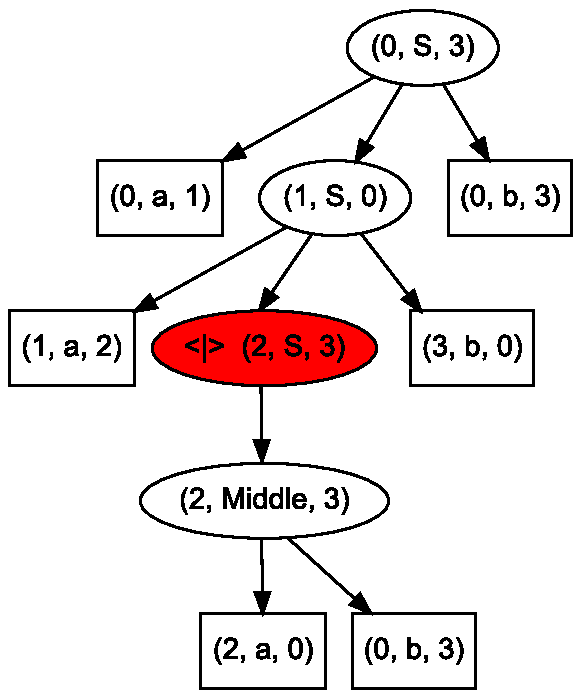
\includegraphics[height=4.5cm]{pictures/AnBn_2.pdf}}
    &
    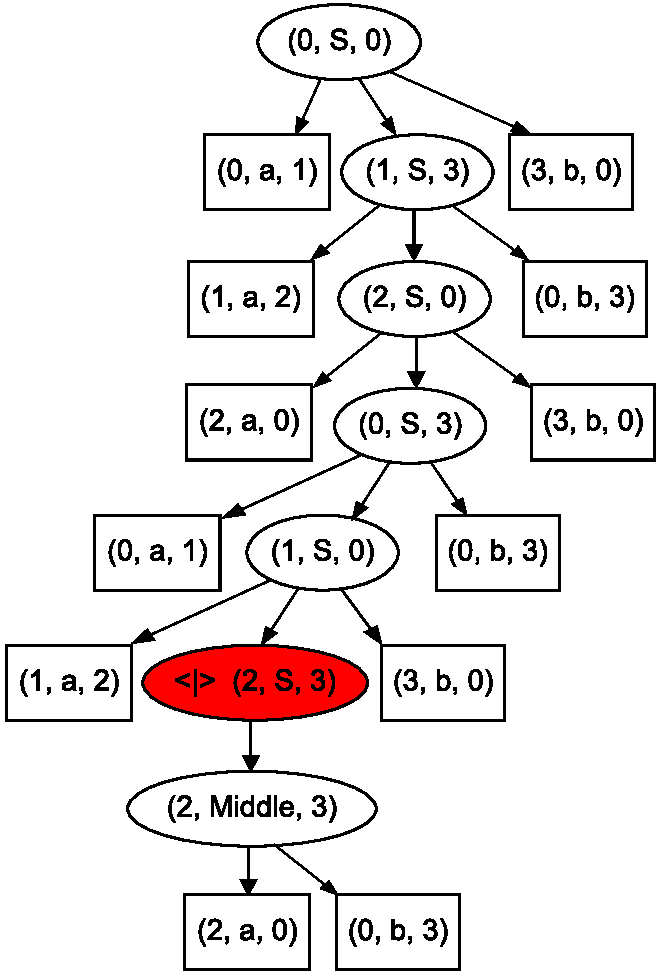
\includegraphics[height=4.5cm]{pictures/AnBn_1.pdf}

\\
\small{Query result: SPPF}
& \small{Tree for the path $0 \leadsto 3$}
& \small{Tree for the path $0 \leadsto 0$}

\end{tabular}
\end{overprint}

\end{frame}

\begin{frame}
  \transwipe[direction=90]
  \frametitle{Our approaches}
  \begin{itemize}
    \item Relaxed parsing of dynamically generated SQL-queries %(\href{https://link.springer.com/chapter/10.1007/978-3-319-41579-6\_22}{Verbitskaia, Grigorev, Avdyukhin. 2015})
%    \begin{itemize}
%        \item Based on RNGLR parsing algorithm (Scott, Johnstone)
%    \end{itemize}
    \item Context-free path querying with structural representation of result %(\href{https://arxiv.org/abs/1612.08872}{Grigorev, Ragozina.~2016})
%    \begin{itemize}
%        \item Based on GLL parsing algorithm (Scott, Johnstone)
%    \end{itemize}
    \item Context-free path querying by matrix multiplication %(\href{https://arxiv.org/abs/1707.01007}{Azimov, Grigorev.~2017})
%    \begin{itemize}
%        \item Inspired by works of Valiant and Okhotin
%    \end{itemize}
    \item Parser combinators for context-free path querying %(\href{http://plc.sfedu.ru/files/PLC-2017-proceedings.pdf\#page=233}{Smolina, Verbitskaia.~2017})
%    \begin{itemize}
%        \item Based on Meerkat: a general parser combinator library for Scala (Afroozeh, Izmaylova)
%    \end{itemize}
  \end{itemize}
\end{frame}

\begin{frame}[fragile]
  \transwipe[direction=90]
  \frametitle{Relaxed parsing of dynamically generated SQL-queries}
  \begin{itemize}
    \item \href{https://link.springer.com/chapter/10.1007/978-3-319-41579-6\_22}{Verbitskaia, Grigorev, Avdyukhin. 2015}
    \item Based on RNGLR parsing algorithm (Scott, Johnstone)
%    \item Specified for string-embedded languages processing
%    \begin{itemize}
%        \item Lexing 
%        \item Heuristics for errors detection and notification
%    \end{itemize}
    \item Static analysis of dynamically generated (SQL)code

        \begin{Verbatim}[commandchars=\\\{\}]
\textcolor{blue}{IF} @X = @Y \textcolor{blue}{SET} @TABLE = \textcolor{orange}{'#table1'}
\textcolor{blue}{ELSE}       \textcolor{blue}{SET} @TABLE = \textcolor{orange}{'table2'}
\textcolor{blue}{EXECUTE} 
    (\textcolor{orange}{'SELECT x FROM '} + @TABLE + \textcolor{orange}{' WHERE ISNULL(n,0) > 1'})
        \end{Verbatim}
     \centering{\huge{$ \Downarrow $}}
                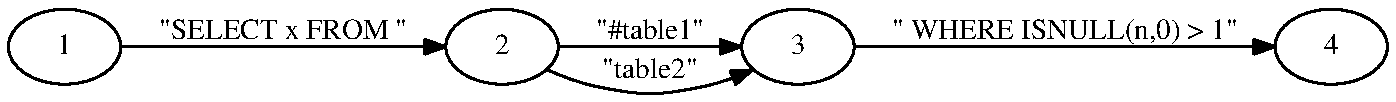
\includegraphics[width = 0.9\textwidth]{pictures/approximation1.pdf} \\
      
  \end{itemize}
\end{frame}

\begin{frame}
  \transwipe[direction=90]
  \frametitle{Context-free path querying with structural representation of result}
  \begin{itemize}
    \item \href{https://arxiv.org/abs/1612.08872}{Grigorev, Ragozina.~2016}
    \item Based on GLL parsing algorithm (Scott, Johnstone)
    \item General-purpose context-free path querying algorithm which can produce user-friendly representation of result
    \item Worst-case space complexity $$O(|V|^3 + |E|)$$
    \item Worst-case time complexity $$O\left(|V|^3*\max\limits_{v \in V}\left(deg^+\left(v\right)\right)\right)$$
%    \item Size of SPPF $O(|V'|^3 + |E'|)$ where $M'=(V',E',L')$ --- подграф $M$, содержащий только искомые пути
  \end{itemize}
\end{frame}

\begin{frame}
  \transwipe[direction=90]
  \frametitle{Context-free path querying by matrix multiplication}
  \begin{itemize}
    \item \href{https://arxiv.org/abs/1707.01007}{Azimov, Grigorev.~2017}
    \item Inspired by works of Valiant and Okhotin    
    \item GPGPU utilization for context-free path querying
    \item Worst-case time complexity $$O(|V|^2 |N|^3 (BMM(|V|) + BMU(|V|)))$$
    \begin{itemize}
      \item BMM --- Boolean Matrix Multiplication
      \item BMU --- Boolean Matrix Union
    \end{itemize}

  \end{itemize}
\end{frame}

\begin{frame}
  \transwipe[direction=90]
  \frametitle{Parser combinators for context-free path querying}
  \begin{itemize}
    \item \href{http://plc.sfedu.ru/files/PLC-2017-proceedings.pdf\#page=233}{Smolina, Verbitskaia.~2017}
    \item Based on Meerkat: a general parser combinator library for Scala (Afroozeh, Izmaylova)
    \item Context-free path querying without DSLs
    \begin{itemize}
    \item May be more friendly for the developers of static code analysis tools
    \item Data-dependent parsing (in progress)
    \end{itemize}
%    \item Size of SPPF $O(|V'|^3 + |E'|)$ where $M'=(V',E',L')$ --- подграф $M$, содержащий только искомые пути
  \end{itemize}
\end{frame}

\begin{frame}[fragile]
\transwipe[direction=90]
\frametitle{Evaluation: data}
\begin{itemize}
\item Graphs ---  the set of ontologies
\item Query is classical ``same-generation query''
\begin{figure}[ht]
   \centering
   \[
\begin{array}{rl}
     & \textbf{S} \rightarrow \text{\textit{subClassOf}}^{-1} \ \textbf{S} \ \text{\textit{subClassOf}} \\ 
     & \textbf{S} \rightarrow \text{\textit{type}}^{-1} \ \textbf{S} \ \text{\textit{type}} \\ 
     & \textbf{S} \rightarrow \text{\textit{subClassOf}}^{-1} \ \text{\textit{subClassOf}} \\ 
     & \textbf{S} \rightarrow \text{\textit{type}}^{-1} \ \text{\textit{type}} \\ 
\end{array}
\]
   \end{figure}

\end{itemize}

\end{frame}


\begin{frame}[fragile]
  \transwipe[direction=90]
  \frametitle{Evaluation: results}
\begin{center}
\rowcolors{1}{}{lightgray}
\begin{tabular}{  c | c | c | c | c  }

Ontology & \#edg & \multicolumn{3}{c}{time (ms)}  \\
\cline{3-5}
& & \shortstack{CYK\footnote{Zhang, et al. ``Context-free path queries on RDF graphs.''}} & \shortstack{GLL} & \shortstack{Matrix} \\
\hline 
\hline
skos           & 252  & 1044    & 10   & 12   \\
generations    & 273  & 6091    & 19   & 13   \\
travel         & 277  & 13971   & 24   & 30   \\
univ-bench     & 293  & 20981   & 25   & 15   \\
people-pets    & 640  & 82081   & 89   & 32   \\
atom-primitive & 425  & 515285  & 255  & 22   \\
\shortstack{biomedical- \\ measure-primitive} 
               & 459  & 420604  & 261  & 20   \\
pizza          & 1980 & 3233587 & 697  & 24   \\
wine           & 1839 & 4075319 & 819  & 54   \\
g1             & 8688 & ---     & 1926 & 82   \\
g2             & 14712 & ---     & 6246 & 185 \\
g3             & 15840 & ---     & 7014 & 127 \\
\end{tabular}
\end{center}
\end{frame}

\begin{frame}[fragile]
\transwipe[direction=90]
\frametitle{Future work: Other grammars and language classes intersection}
  \begin{itemize}
     \item Context-free grammars intersection: Nederhof, ``The language intersection problem for non-recursive context-free grammars''
     \begin{itemize}  
       \item Compressed strings processing
       \item Grammar-compressed graphs querying
     \end{itemize}
     \item Approximated intersection of regular and conjunctive/boolean languages
     \begin{itemize}  
       \item More expressive query languages
%       \item More tasks (POPL-2017)
     \end{itemize}
     \item \dots
  \end{itemize}
\end{frame}

\begin{frame}[fragile]
\transwipe[direction=90]
\frametitle{Future work: Mechanization in Coq}
\begin{itemize}
%  \begin{itemize}
     \item Bar-Hillel theorem
     \item GLL-based algorithms
     \item Other algorithms for grammars intersection
%  \end{itemize}
\end{itemize}
\begin{itemize}
%  \begin{itemize}
     \item Basic (parsing) algorithms verification
     \item Base for complex algorithms verification
%  \end{itemize}
\end{itemize}


\end{frame}

            
\begin{frame}
\transwipe[direction=90]
\frametitle{Contact information}
\begin{itemize}
  \item Semyon Grigorev: \href{mailto:semen.grigorev@jetbrains.com}{semen.grigorev@jetbrains.com}
  \item Kate Verbitskaia: \href{mailto:ekaterina.verbitskaya@jetbrains.com}{ekaterina.verbitskaya@jetbrains.com}
\end{itemize}
\begin{itemize}
  \item YaccConstructor: \href{https://github.com/YaccConstructor}{https://github.com/YaccConstructor}
\end{itemize}
\end{frame}
\end{document}
